\documentclass{article}
\usepackage{graphicx}
\usepackage{amsmath}
\usepackage{subcaption}


\title{3D Data Processing: Point Cloud Registration}
\author{Pooya Nasiri \thanks{Email: pooya.nasiri@studenti.unipd.it | Matricola 2071437}}
\date{June 1, 2024}

\begin{document}

\maketitle

\section{Introduction}
The objective of this assignment is to implement the Iterative Closest Point (ICP) algorithm to find the fine alignment transformation between a source and a target point cloud. The assignment involved modifying the provided C++ software to complete the ICP main loop, closest point matching, and transformation matrix estimation.

%\section{Implementation Details}
%The implementation focused on completing the following methods in the \texttt{registration.cpp} file:

%\begin{itemize}
%    \item \texttt{find\_closest\_point(...)}: This method finds the closest points in the target cloud for each point in the source cloud using a KD-Tree for efficient nearest neighbor search.
%    \item \texttt{get\_svd\_icp\_registration(...)}: This method computes the transformation matrix using Singular Value Decomposition (SVD). It involves calculating centroids of the point clouds, constructing a covariance matrix, and performing SVD to obtain the optimal rotation and translation.
%    \item \texttt{get\_lm\_icp\_registration(...)}: This method uses the Levenberg-Marquardt (LM) algorithm implemented in Ceres Solver to optimize the transformation parameters. A custom cost function was defined to minimize the distance between the transformed source points and the target points.
%    \item \texttt{execute\_icp\_registration(...)}: This is the main ICP loop that iteratively calls the closest point matching and transformation estimation methods, checking for convergence based on the Root Mean Square Error (RMSE).
%\end{itemize}


\section{Implementation Details}
The implementation focused on completing the following methods \newline in the \texttt{registration.cpp} file:

\subsection{find\_closest\_point(...)}
This method finds the closest points in the target cloud for each point in the source cloud. The KD-Tree data structure from the Point Cloud Library (PCL) is used for efficient nearest neighbor search.

\begin{itemize}
    \item \textbf{KD-Tree Construction:} The target point cloud is used to construct the KD-Tree.
    \item \textbf{Nearest Neighbor Search:} For each point in the source cloud, the nearest neighbor in the target cloud is found using the KD-Tree.
    \item \textbf{Output:} The method returns the indices of the closest points in the target cloud.
\end{itemize}

\subsection{get\_svd\_icp\_registration(...)}
This method computes the transformation matrix using Singular Value Decomposition (SVD).

\begin{itemize}
    \item \textbf{Centroid Calculation:} The centroids of both the source and target point clouds are calculated.
    \item \textbf{Covariance Matrix:} A covariance matrix is constructed using the centered coordinates of the point clouds.
    \item \textbf{SVD Computation:} SVD is performed on the covariance matrix to obtain the rotation matrix.
    \item \textbf{Translation Vector:} The translation vector is computed using the centroids and the rotation matrix.
    \item \textbf{Transformation Matrix:} The final transformation matrix is assembled from the rotation matrix and translation vector.
\end{itemize}

\subsection{get\_lm\_icp\_registration(...)}
This method uses the Levenberg-Marquardt (LM) algorithm, implemented in the Ceres Solver, to optimize the transformation parameters.

\begin{itemize}
    \item \textbf{Cost Function:} A custom cost function is defined to minimize the Euclidean distance between the transformed source points and the target points.
    \item \textbf{Parameter Initialization:} The initial parameters (rotation and translation) are set.
    \item \textbf{Optimization:} The LM optimizer is run to refine the transformation parameters.
    \item \textbf{Output:} The optimized transformation matrix is returned.
\end{itemize}

\subsection{execute\_icp\_registration(...)}
This is the main ICP loop that iteratively calls the closest point matching and transformation estimation methods.




\section{Results}
The ICP algorithm was tested on the provided datasets, and the following results were obtained:

\subsection{Qualitative Results}
Figures \ref{fig:point_clouds} show the initial and aligned point clouds for the two datasets. The source cloud is colored in orange, and the target cloud is colored in blue.


\begin{figure}[h!]
    \centering
    \begin{subfigure}[b]{0.3\textwidth}
        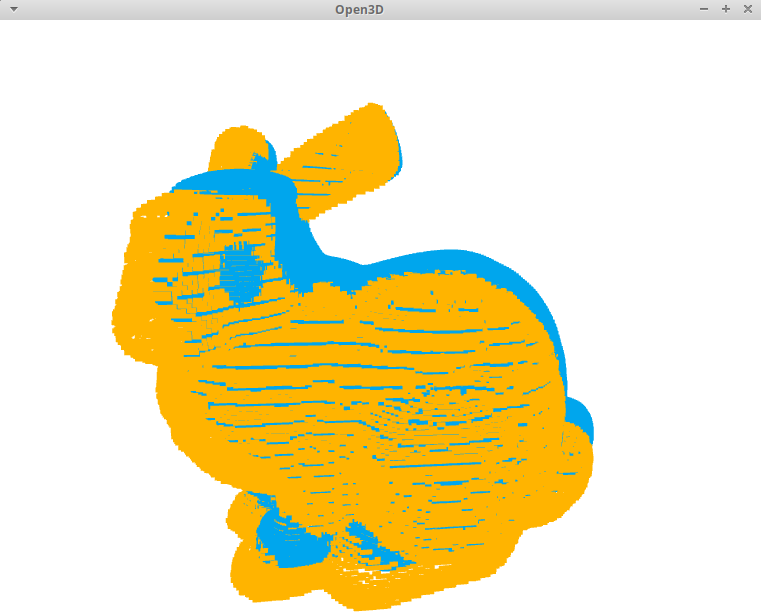
\includegraphics[width=\textwidth]{bunny1.png}
        \caption{Initial point clouds for Bunny.}
    \end{subfigure}
    \begin{subfigure}[b]{0.3\textwidth}
        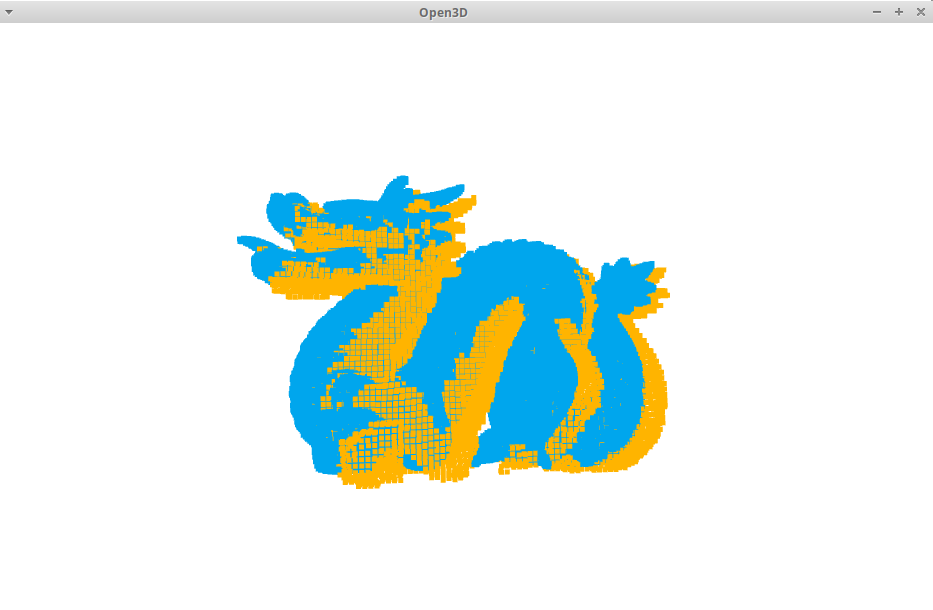
\includegraphics[width=\textwidth]{dragon1.png}
        \caption{Initial point clouds for Dragon.}
    \end{subfigure}
    \begin{subfigure}[b]{0.3\textwidth}
        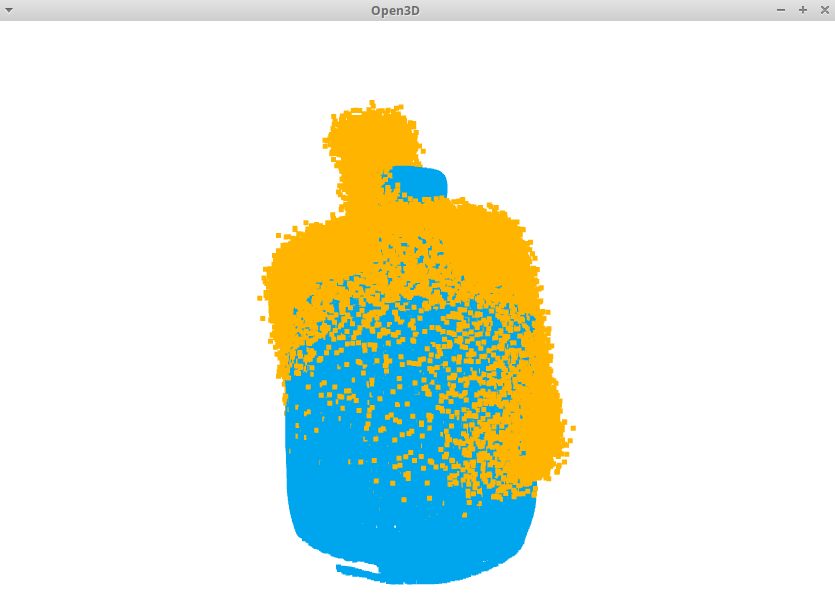
\includegraphics[width=\textwidth]{vase1.png}
        \caption{Initial point clouds for Vase.}
    \end{subfigure}

    \begin{subfigure}[b]{0.3\textwidth}
        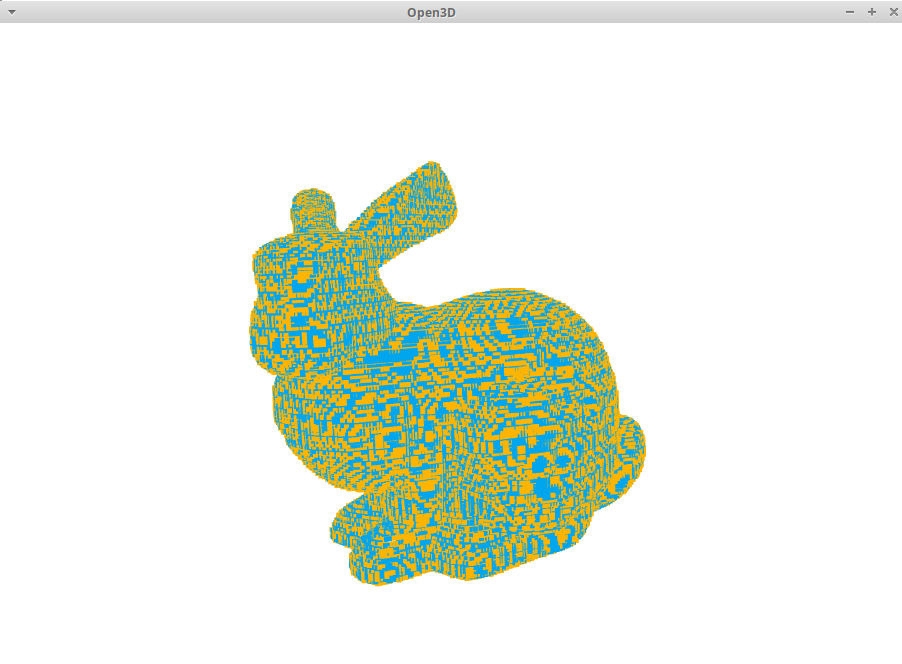
\includegraphics[width=\textwidth]{bunny2.png}
        \caption{Aligned point clouds for Bunny.}
    \end{subfigure}
    \begin{subfigure}[b]{0.3\textwidth}
        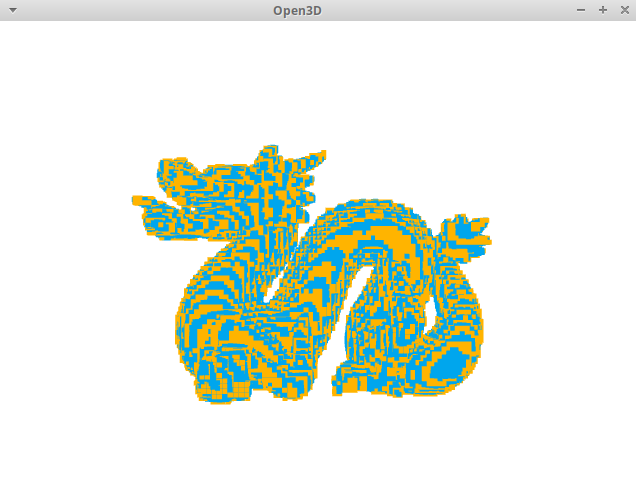
\includegraphics[width=\textwidth]{dragon2.png}
        \caption{Aligned point clouds for Dragon.}
    \end{subfigure}
    \begin{subfigure}[b]{0.3\textwidth}
        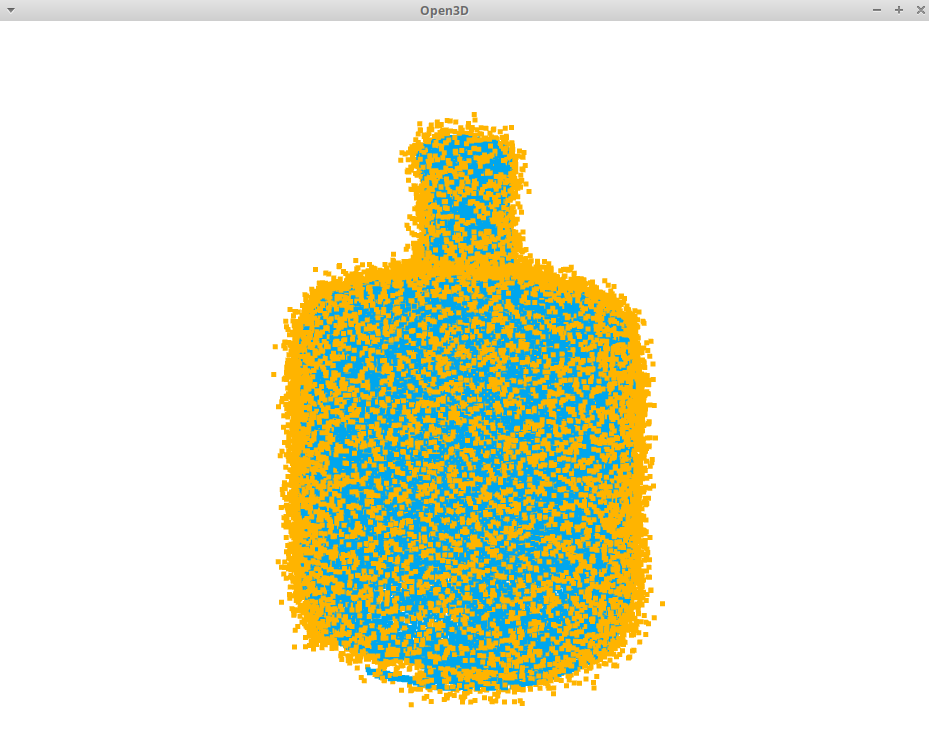
\includegraphics[width=\textwidth]{vase2.png}
        \caption{Aligned point clouds for Vase.}
    \end{subfigure}

    \caption{Initial and aligned point clouds for Bunny, Dragon, and Vase datasets.}
    \label{fig:point_clouds}
\end{figure}


\subsection{Quantitative Results}
The RMSE values for the aligned point clouds were computed to quantify the accuracy of the registration:

\begin{table}[h!]
    \centering
    \begin{tabular}{|c|c|c|c|}
        \hline
        \textbf{Dataset} & \textbf{Initial RMSE} & \textbf{Final RMSE} & \textbf{Iterations} \\
        \hline
        Bunny & 0.045392 & 0.00341366 & 20 \\
        \hline
        Vase & 0.0714058 & 0.0162217 & 28 \\
        \hline
        Dragon & 0.0276689 & 0.00564134 & 18 \\
        \hline
    \end{tabular}
    \caption{RMSE reduction and iterations for different datasets}
    \label{tab:rmse_iterations}
\end{table}


\section{Conclusion}
The ICP algorithm was successfully implemented, achieving fine alignment between the source and target point clouds. The qualitative results visually confirm the alignment, and the quantitative RMSE values provide a measure of the accuracy.

\end{document}
